\documentclass[../entwurf.tex]{subfiles}
\begin{document}
\section{Architektur}
\begin{center}
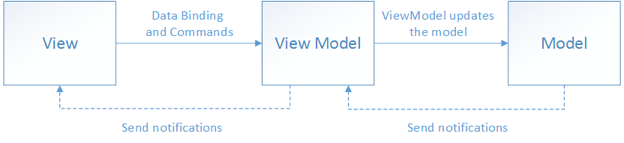
\includegraphics[scale=0.8]{../graphics/mvvm.png}
\textit{MVVM-Architektur\footnote{\tiny{https://docs.microsoft.com/de-de/xamarin/xamarin-forms/enterprise-application-patterns/mvvm}}}
\end{center}

Die Grundstruktur der Anwendung basiert auf der MVVM-Architektur. Dabei soll das Viewmodel das Model von der View isolieren. Diese Dreiteilung der Komponenten ermöglicht Entwicklern, das Model unabhängig von der View zu entwickeln. Außerdem kann durch die lose Kopplung der Komponenten die Benutzeroberfläche der Anwendung ohne Berühren des Codes umgestaltet werden. Die drei Komponenten sollen dabei folgende  Aufgaben erfüllen.
\newline
\newline
\code{Model}
\newline
Diese Komponente enthält die gesamte Geschäftslogik und stellt die Datenzugriffsschicht für die Inhalte, die dem Benutzer angezeigt und von ihm manipuliert werden dar. Dazu benachrichtigt sie über Datenänderungen empfängt vom Benutzer übergebenen Daten.
\newline
\newline
\code{View}
\newline
Diese Komponente enthält alle Elemente des GUIs. Sie bindet sich an Eigenschaften des Viewmodels, um Inhalte darzustellen sowie Benutzereingaben/-aktionen weiterzuleiten. Durch die Datenbindung ist die View einfach austauschbar und ihr Code-Behind gering.
\newline
\newline
\code{Viewmodel}
\newline
Diese Komponente enthält die UI-Logik und dient als Bindeglied zwischen View und Model. Einerseits tauscht sie Information mit dem Model aus, andererseits stellt sie der View Eigenschaften und Befehle zur Verfügung.  Das ViewModel hat dabei keinerlei Kenntnis der View.

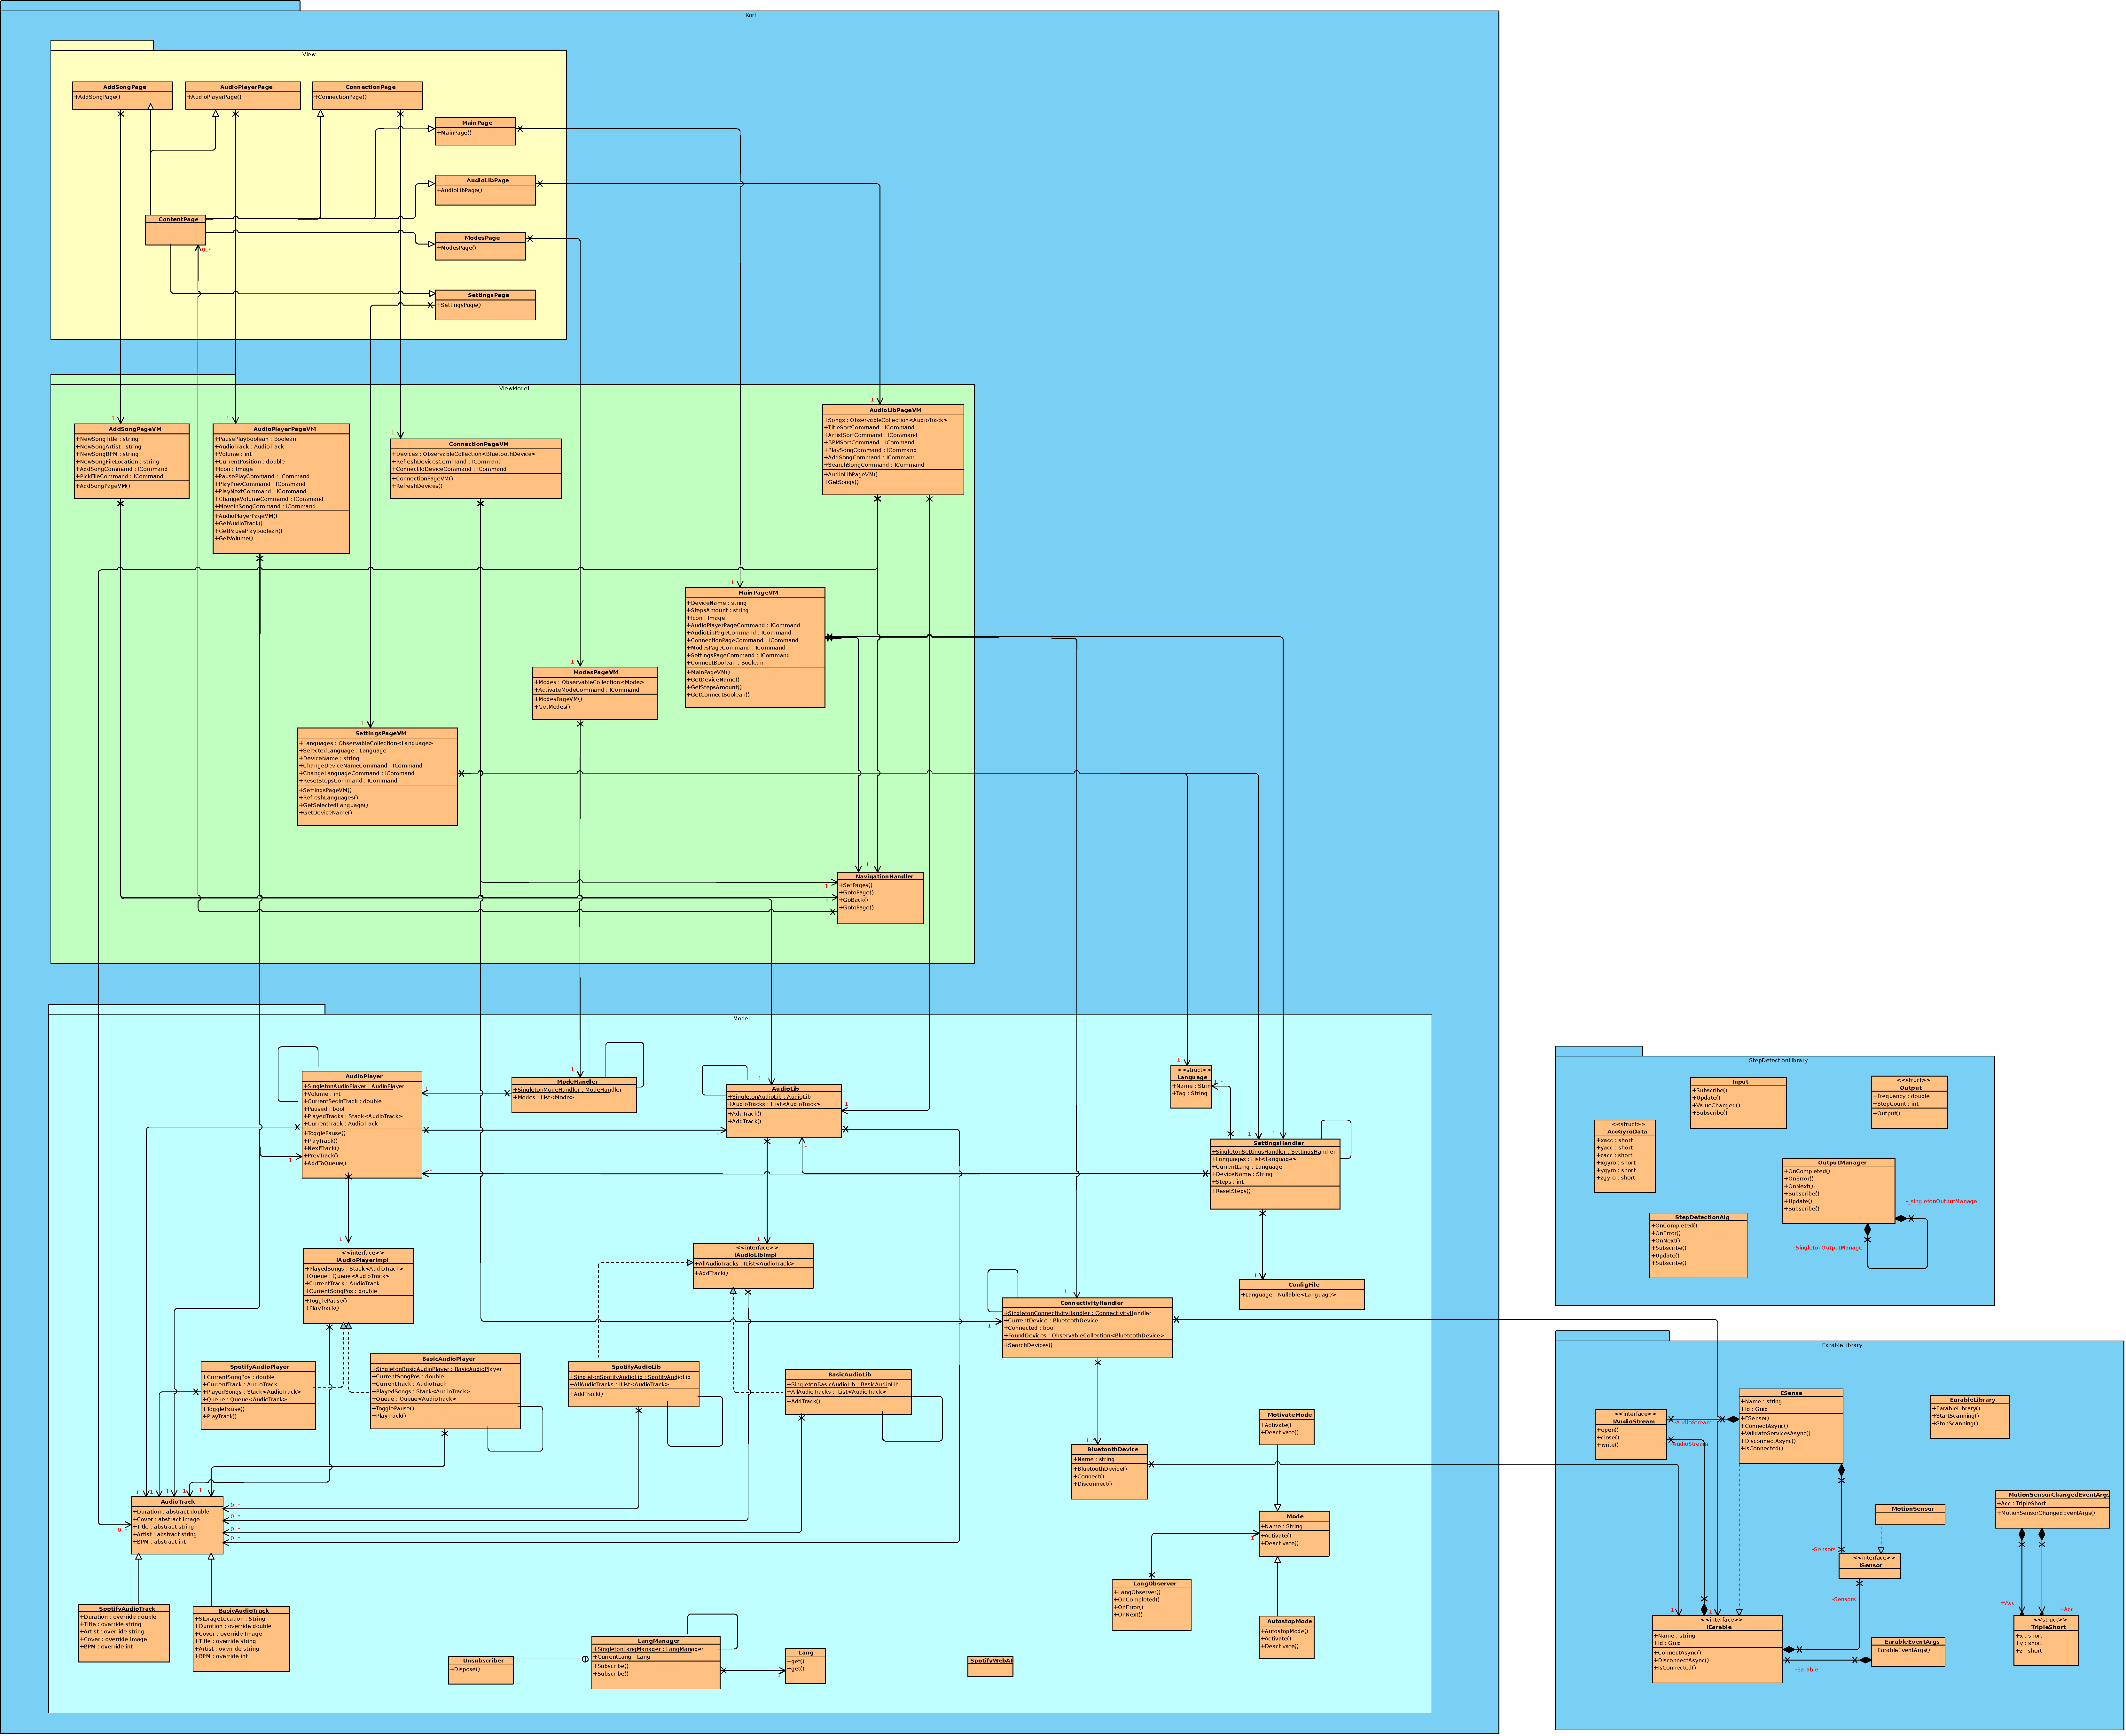
\includepdf[scale=0.8,pages=1,pagecommand=\section{UML-Klassendiagramm}\textit{Siehe Anhang für eine detailliertere Version}]{../graphics/uml_diagramme/Gesamt.pdf}

\end{document}
